\section{Dinámicas especiales}

\subsection{Canales de Pauli}

\acnote{Cambiar la probabilidad $p$ por otra cosa, que se estorba con la $p$ del CG}

Los canales de Pauli son canales cuánticos en los que se aplica un operador de Pauli con alguna probabilidad. El canal de Pauli de un qubit más general está definido como
\begin{gather}
    P:\mcB(\hilbert_{2}) \rightarrow \mcB(\hilbert_{2})\nonumber\\
    P(\Delta)=\sum_{j=0}^{3}p_{j}\pauli{j}\Delta\pauli{j}\rlap{.}\nonumber
\end{gather}
Reconociendo que cualquiera de los tres operadores de Pauli puede escribirse en términos de los otros dos, se puede aprovechar la relación $-i\pauli{2}=\pauli{1}\pauli{3}$, para escribir a los canales de Pauli de una forma particularmente útil:
\begin{equation}
    P(\Delta)=\sum_{j,k=0}^{1}p_{j,k}\pauli{1}^{j}\pauli{3}^{k}\Delta\pauli{3}^{k}\pauli{1}^{j}.\nonumber
\end{equation}
A través de esta expresión se extienden los canales de Pauli de un qubit a $n$ qubits como
\begin{gather}
    P:\mcB(\hilbert_{2^{n}}) \rightarrow \mcB(\hilbert_{2^{n}})\nonumber\\
    P(\Delta)=\sum_{\vec{j},\vec{k}}p_{\vec{j},\vec{k}}\pauli{1}^{\vec{j}}\pauli{3}^{\vec{k}}\Delta\pauli{3}^{\vec{k}}\pauli{1}^{\vec{j}}\rlap{.}\nonumber
\end{gather}
donde $\pauli{j}^{\vec{k}}=\pauli{j}^{k_{1}}\otimes\pauli{j}^{k_{2}}\otimes ... \otimes \pauli{j}^{k_{n}}$ y las entradas $k_{l}$ del vector $\vec{k}$ solo pueden valer $0$ o $1$.

\subsubsection{Canales de desfasamiento}

Por canales de desfasamiento se entiende aquellos canales cuánticos cuyo efecto es amortiguar los elementos fuera de la diagonal del operador sobre el que actúan. Ahora, esta definición es dependiente de la base sobre la que se está trabajando. Por ejemplo, sea $\rho\in\densityspace{2}$. Si se utiliza la base de eigenestados de $\pauli{3}$, entonces el canal
\begin{equation}
    \rho\mapsto p_{1}\rho + p_{2} \pauli{3}\rho\pauli{3}\nonumber
\end{equation}
es un canal de desfasamiento, mientras que el canal de \textit{bit flip},
\begin{equation}
    \rho\mapsto p_{1}\rho + p_{2} \pauli{1}\rho\pauli{1},\nonumber
\end{equation}
no lo es. Por supuesto, el canal de \textit{bit flip} es un canal de desfasamiento si se trabaja en la base de los eigenestados de $\pauli{1}$. Para extender los canales de desfasamiento a $n$ qubits, primero nótese que
\begin{equation}
    \Motimes \ket{e_{j}}
\end{equation}
con $\{\ket{e_{j}}\}$ una base de $\hilbert_{n}$, es una base de $\hilbert_{2^{n}}$. Esto significa que podemos utilizar productos tensoriales de los eigenestados de \acnote{eh}


Así, podemos estudiar dos canales de desfasamiento, el primero actuando en la base de productos tensoriales de eigenestados de $\pauli{3}$,
\begin{gather}
    P_{\pauli{3}}:\mcB(\hilbert_{2^{n}}) \rightarrow \mcB(\hilbert_{2^{n}})\nonumber\\
    P_{\pauli{3}}(\Delta)=\sum_{\vec{k}}p_{\vec{k}}\pauli{3}^{\vec{k}}\Delta\pauli{3}^{\vec{k}}\rlap{.}\nonumber
\end{gather}
y el segundo sobre la base de productos tensoriales de eigenestados de $\pauli{1}$,
\begin{gather}
    P_{\pauli{1}}:\mcB(\hilbert_{2^{n}}) \rightarrow \mcB(\hilbert_{2^{n}})\nonumber\\
    P_{\pauli{1}}(\Delta)=\sum_{\vec{j}}p_{\vec{j}}\pauli{1}^{\vec{j}}\Delta\pauli{1}^{\vec{j}}\rlap{.}\nonumber
\end{gather}
 Si se escoje $p_{\vec{j}}=\frac{1-p_{\vec{0}}}{n-1}\,\forall\,\vec{j}\neq\vec{0}$, el efecto de estos canales es de reducir la amplitud de las componentes fuera de la diagonal por un factor de $(2p_{1}-1)$

Consideremos en canal de desfasamiento de dos qubits en dirección $a$ con probabilidades como mencionadas anteriormente. Si se propaga al estado de máxima entropía por medio de este canal y luego se aplica el centering


\subsubsection{Canal de despolarización}

El canal de despolarización no es más que un canal de Pauli con distribución uniforme en las probabilidades \acnote{arreglar}

Consideremos una evolución subyacente no unitaria: el canal de despolarización. El canal de despolarización para $n$ partículas está definido como
\begin{equation*}
    D_{\mu}(\varrho)=\mu\varrho+(1-\mu)\Id.
\end{equation*}
Dado un estado efectivo inicial $\rho$, su asignación de máxima entropía es $\varrho_{\max}=\rho_{A}\otimes\rho_{B}$. El resultado de pasar al estado de máxima entropía por el canal de despolarización es simplemente
\begin{equation*}
    D_{\mu}(\varrho_{\max})=\mu\varrho_{\max}+(1-\mu)\Id.
\end{equation*}
Esto significa que la dinámica efectiva es
\begin{equation*}
    \Gamma_{t=1}(\rho)=\mu\rho+(1-\mu)\Id,
\end{equation*}
esto es, ¡el mismo canal de despolarización aplicado a un sistema de menos partículas! Nótese que este resultado es muy similar al obtenido para una evolución unitaria subyacente generada por un Hamiltoniano de la forma $\mcH=H\otimes\Id+\Id\otimes H$. En dicho caso, la dinámica efectiva era, justamente, la unitaria generada por el Hamiltoniano $H$, esto como consecuencia de la simetría de la evolución: la misma para cada partícula, sin interacción. Este caso es el mismo, el canal de despolarización actúa de la misma forma sobre cada partícula, y es completamente isotrópico dentro del subespacio de cada partícula.

\subsection{Amortiguamiento de amplitud}

\subsection{Estabilización espontánea ?}
Considérese que un sistema de $n$ partículas evoluciona siguiendo el canal
\begin{equation*}
    \mcE_{\psi,t}[\varrho]=e^{-t\mu}\varrho+(1-e^{-t \mu})\dyad{\psi}
\end{equation*}
donde $\dyad{\psi}\in \densityspace{n}$. Aplicando el modelo de grano grueso se obtiene que:
\begin{equation*}
    \rho(t)=e^{-t\mu}\rho(0)+(1-e^{-t \mu})\dyad{\psi}_{eff}
\end{equation*}
donde $\dyad{\psi}_{eff}=\mcC(\dyad{\psi})$. Obsérvese que el resultado es un canal del mismo tipo. La única diferencia siendo que el estado al que el sistema \textit{decae} (abusando del lenguaje) es la descripción efectiva de $\dyad{\psi}$. Como es natural, el comportamiento de la evolución es completamente dependiente de $\psi$, pero, al fin y al cabo, ¡se obtiene un canal cuántico!

\subsection{Modelo de Ising}

El Hamiltoniano del modelo de Ising transversal es
\begin{equation*}
    H=-\omega\qty(\sum_{\langle j,k \rangle}\pauli{3,j}\otimes\pauli{3,k}+g\sum_{k}\Id\otimes\pauli{1,k}),
\end{equation*}

que, si $g=0$ (fase ordenada) y tomando en cuenta únicamente un par de partículas se convierte en el Hamiltoniano de interacción
\begin{equation*}
    H=-\omega \pauli{3}\otimes\pauli{3}.
\end{equation*}

Dado un estado efectivo $\rho\in\densityspace{2}$, propagar al estado asignando a través del Principio de Máxima Entropía con dicha evolución y luego tomar la descripción dada por la aplicación de grano grueso resulta en la dinámica efectiva
\begin{align*}
    \Gamma_{t}^{p}(\rho)=&\rho \cos^{2}(\omega)+\pauli{3} \rho \pauli{3} \sin^{2}(\omega t)\\
    & + i\sin(\omega t)\cos(\omega t)\qty(p\expval{\pauli{3}}_{B}[\pauli{3},\rho_{A}]+(1-p)\expval{\pauli{3}}_{A}[\pauli{3},\rho_{B}]).
\end{align*}
Reconocemos dos términos: uno lineal y uno no lineal. El primero tiene forma de canal de desfasamiento sobre el estado efectivo. El segundo depende de los parámetros de la aplicación de grano grueso y de los valores esperados con respecto a los operadores de densidad reducidos del estado de máxima entropía. En efecto, el caso límite $p=1$ o $p=1$ simplemente reduce la dinámica a un canal de desfasamiento:

\begin{equation*}
    \Gamma_{t}^{p=1}(\rho)=\rho \cos^{2}(\omega)+\pauli{3} \rho \pauli{3} \sin^{2}(\omega t).
\end{equation*}

mientras que el caso $p=\frac{1}{2}$ revela el efecto del término no lineal:

\begin{equation*}
    \Gamma_{t}^{p=\frac{1}{2}}(\rho)=\rho \cos^{2}(\omega)+\pauli{3} \rho \pauli{3} \sin^{2}(\omega t) + i\expval{\pauli{3}} \qty[\pauli{3},\rho] \sin(\omega t)\cos(\omega t).
\end{equation*}

Nótese que, si del factor $\expval{\pauli{3}}=1$, la dinámica sería no solo lineal, sino unitaria, y correspondería a una rotación respecto al eje $z$, de no ser que los únicos estados tales que $\expval{\pauli{3}}=1$ son invariantes bajo dichas rotaciones. En realidad, lo que se observa es que la dinámica efectiva es una rotación respecto a $z$ que depende de la componente en $z$ del estado efectivo inicial. Cuando $\expval{\pauli{3}}=0$, la dinámica es un canal de despolarización que manda a todos los estados al eje $z$ (a un tiempo $\omega t =\frac{\pi}{4}$). 

\begin{figure}[ht!]
    \centering
    \begin{subfigure}{0.32\textwidth}
      \centering
      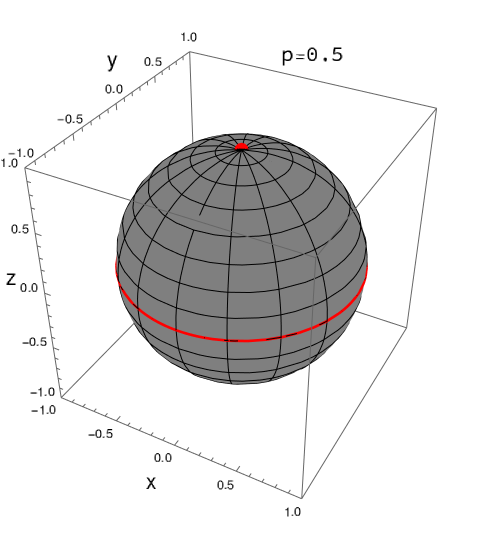
\includegraphics[width=0.9\linewidth]{chapter3/figures_special/sphere_Ising_t=0._z=0.9_p=0.5.png}
      \caption{$t=0$}
    \end{subfigure}%
    \begin{subfigure}{0.32\textwidth}
      \centering
      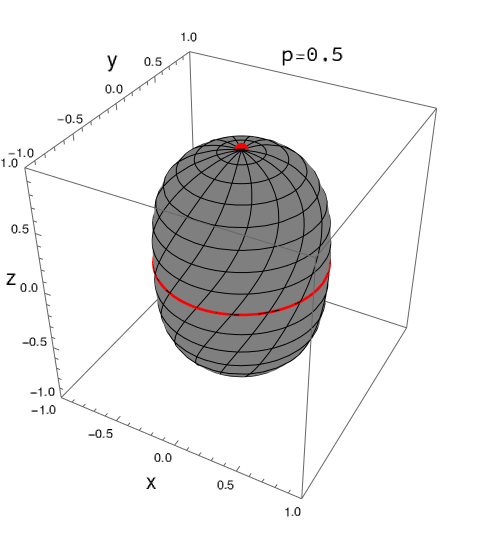
\includegraphics[width=0.9\linewidth]{chapter3/figures_special/sphere_Ising_t=0.5_z=0.9_p=0.5.png}
      \caption{$t=0.5$}
    \end{subfigure}
    \begin{subfigure}{0.32\textwidth}
      \centering
      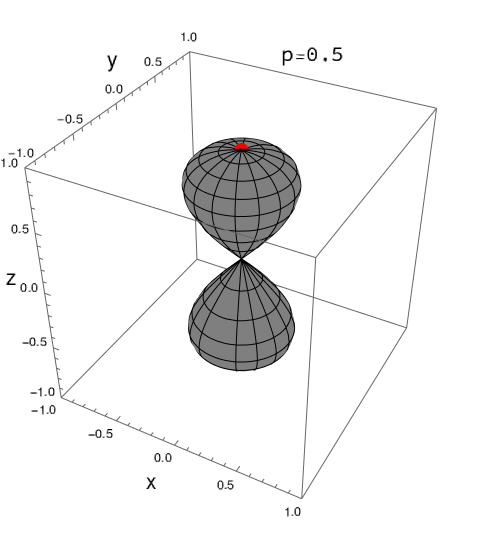
\includegraphics[width=0.9\linewidth]{chapter3/figures_special/sphere_Ising_t=1._z=0.9_p=0.5.png}
      \caption{$t=1$}
    \end{subfigure}
    \caption{Efecto del la evolución sobre la esfera de Bloch cuando $p=\frac{1}{2}$. Nótese que el desfasamiento sólo se completa en el eje $xy$.}
    \label{fig:Ising_p0.5_Sequence}
    \end{figure}

La despolarización dependiente de la componente en $z$ inicial es más clara si se observa el efecto de la evolución sobre el vector de Bloch. Abusando un poco de la notación se nota que 

\begin{equation*}
    \Gamma_{t}^{p=\frac{1}{2}}(\vec{r}_{\rho})=\begin{pmatrix}
        x\cos(2\omega t)-yz\sin(2\omega t)\\
        y\cos(2\omega t)+xz(2\omega t)\\
        z\\
    \end{pmatrix}
\end{equation*}
\acnote{Aquí se ve la casi rotación, pero creo que lo tengo que descomponer en diferentes operaciones para notar que el desfasamiento se da de forma más fuerte conforme más pequeño es z}
